\documentclass[12pt, a4paper]{article}

% Preamble
\usepackage{xeCJK}
\usepackage[utf8]{inputenc}
\usepackage[english]{babel}
\usepackage[margin=1in]{geometry}
\usepackage[parfill]{parskip}
\usepackage{listings}
\usepackage{graphics}
\usepackage{graphicx}
\usepackage{nasm/lang}
\usepackage{nasm/style}
\usepackage{c/style}
\usepackage{go/lang}
\usepackage{go/style}
\usepackage{reil/lang}
\usepackage{llvm/lang}
\usepackage{diff/lang}
\usepackage{diff/style}
\usepackage{dot/lang}
\usepackage{dot/style}
\usepackage{float}
\usepackage[colorlinks,linkcolor=blue]{hyperref}
\usepackage{listings}
\lstset{basicstyle={\normalfont\sffamily},breaklines}

\title{开题报告}
\author{Rust-FreeRTOS Team}
\date{March 28, 2019}

\begin{document}
	\maketitle
	\clearpage
	\tableofcontents
	\clearpage
	\section{项目背景}
	计算机发展至今,随着摩尔定律,硬件发展已经达到了一些瓶颈。从而诞生了一些问题:软件的演进速度大大低于硬件的演进。软件在语言级别上无法真正利用多核计算带来的性能提升。而Rust语言是针对多核体系提出的语言,并且吸收一些其他动态语言的重要特性,比如不需要管理内存,比如不会出现Null指针等等。
	
	同时Rust语言系统设计于保证内存安全,它在安全代码里不允许空指针,悬垂指针和数据竞争。数值只能用一系列固定形式来初始化,要求所有输入已经被初始化。在其它语言中复制函数指针或者有效或者为空,比如在链表和二叉树等数据结构中,Rust核心库提供Option类型,用来测试指针是否有值。Rust同时引入添加语法来管理生命周期,而且编译器通过租借检查器来说明相关理由。这些都保证了Rust语言极高的安全性。
	
	在嵌入式领域中,嵌入式实时操作系统正得到越来越广泛的应用。采用嵌入式实时操作系统(RTOS)可以更合理、更有效地利用CPU的资源。FreeRTOS则是一个轻量级的操作系统,可基本满足较小系统的需要。而现今嵌入式系统不断得到更加广泛的使用,人们对于RTOS的可靠性和安全性也有了更高的要求。
	\section{立项依据}
	\subsection{C语言安全性问题与Rust的可靠性}
	众所周知,众多操作系统内核都是由C语言编写而成的,但是由于设计原因,C语言有灵活高效的指针操作,但是这些使得它的安全性不能保证,主要体现在:
	
\textbf{- 空指针引用(NULL Dereference)\\
		- 释放内存后再使用(Use After Free)\\
		- 返回悬空指针(Dangling Pointers)\\
		- 超出访问权限(Out Of Bounds Access)}
	
	声名狼藉的\textbf{程序分段错误(Segmentation Fault)}是C语言的常见问题,而通常NULL dereferences是第一大诱因。如果开发者忘记了检查所返回的指针是否正确性,就可能会导致空指针引用。Rust处理这类指针错误的方式非常极端,在“安全”代码中粗暴简单地禁用所有裸指针。此外在“安全”代码中,Rust还取消了空值。
	
	像C++一样,Rust也使用\textbf{资源获取即初始化(Resource Acquisition Is Initialization)的方式},这意味着每个变量在超出范围后都一定会被释放,因此在“安全的”Rust代码中,永远不必担心释放内存的事情。但Rust不满足于此,它更进一步,直接禁止用户访问被释放的内存。这一点通过Ownership规则实现,在Rust中,变量有一个所有权(Ownership)属性,owner有权随意调用所属的数据,也可以在有限的lifetime内借出数据(即Borrowing)。此外,数据只能有一个owner,这样一来,通过RAII规则,owner的范围指定了何时释放数据。最后,ownership还可以被“转移”,当开发者将ownership分配给另一个不同的变量时,ownership就会转移。
	
	C语言老手都知道,向\textbf{stack-bound变量返回指针很糟糕}, 返回的指针会指向\textbf{未定义内存}。虽然这类错误多见于新手,一旦习惯堆栈规则和调用惯例,就很难出现这类错误了。事实证明,Rust的lifetime check不仅适用于本地定义变量,也适用于返回值。与C语言不同,在返回reference时,Rust的编译器会确保相关内容可有效调用,也就是说,编译器会核实返回的reference有效。即Rust的reference总是指向有效内存。
	
	另一个常见问题就是在访问时,访问了没有权限的内存,多半情况就是所访问的数组,其索引超出范围。这种情况也出现在读写操作中,访问超限内存会导致可执行文件出现严重的漏洞,这些漏洞可能会给黑客操作你的代码大开方便之门。著名的就是\href{https://tonyarcieri.com/would-rust-have-prevented-heartbleed-another-look}{Heartbleed bug}问题。
	
	\subsection{Rust并发模型}
	对于一个操作系统,我们有相当关注这些问题:异步、无锁、并发。
	
	Rust语言项目初始是为了解决两个棘手问题:
	\begin{enumerate}
	\item 如何进行安全的系统编程?
	
	\item 如何实现无痛苦的并发编程?
	\end{enumerate}
	最初,这些问题似乎是正交的不相关,但是让我们惊讶的是,最终解决方案被证明是相同的:同样使Rust安全的工具也帮助你正面解决并发。
	
	内存的安全错误和并发错误往往归结为代码访问数据引起的问题,这是不应该的。Rust秘密武器是ownership,系统程序员需要服从的访问控制纪律,Rust编译器也会为你静态地检查。
	
	对于内存安全,意味着你在一个没有垃圾回收机制下编程,不用害怕segfault,因为Rust会抓住这些错误。
	
	对于并发,这意味着你可以选择各种各样的并发范式(消息传递、共享状态、无锁、纯函数式),而Rust会帮助你避免常见的陷阱。
	
	下面是Rust的并发风格:
	
	\begin{itemize}
	\item channel只传送属于其的消息,你能从一个线程发送指针到另外一个线程,而不用担心这两个线程因为同时访问这个指针产生竞争争夺,Rust的channel通道是线程隔离的。
	\item lock知道其保护数据,当一个锁被一个线程hold住,Rust确保数据只能被这个线程访问,状态从来不会意外地被分享,\textbf{锁住数据,而不是代码 是Rust特点}
	\item 每个数据类型都能知晓其是否可以在多线程之间安全传输或访问,Rust增强这种安全用途;也就没有数据访问争夺,即使对于无锁的数据结构,线程安全不只是文档上写写,而是其实在的法律规则。
	\item 你能在线程之间分享stack frames, Rust会确保这个frame在其他线程还在使用它时一直活跃,\textbf{在Rust中即使最大胆的共享也会确保安全。}
	\end{itemize}
	
	所有这些好处都是得益于Rust的所有权模型,和事实上锁、通道channel和无锁数据结构等之类的库包,这意味着Rust的并发目标是开放的,新的库包对新的范式编程更有力,也能捕获更多bug,这些都只要使用Rust的所有权特性来增加拓展API。
	
	Rust的并发编程模型保证了:\textbf{编译器阻止了所有的数据竞争}
	
	\textbf{A data race is any unsynchronized, concurrent access to data involving a write.}
	
	上面这句话中的同步包括底层的原子指令。它本质上说明了你不能在线程间意外地共享状态,状态的所有(可变)访问都需要以某种同步方式进行。
	
	数据竞争只是一种(非常重要)竞争(race condition),但是通过阻止它,Rust经常帮助你有效地阻止其他的,更加微妙的竞争。举个例子,把不同位置的数据更新弄成原子操作是很重要的:其他线程要么能看到所有更新,要么一个更新也看不到。在Rust中,同时拥有相关位置的\textbf{mut}引用,将保证对他们的更新是原子的。因为不可能会有其他的线程能同时访问。许多语言通过垃圾回收来保障内存安全。但是垃圾回收并没有在阻止数据竞争方面给你提供任何帮助。
	
	Rust则用ownership和borrowing来实现它的两个关键的价值观:
	\begin{enumerate}
	\item  没有垃圾回收的内存安全
	\item  没有数据竞争的并发
	\end{enumerate}

	\subsection{Rust的高效性}
	作为新生的编程语言,我们关注问题之一就是他的性能。虽然不能说Rust再所有环境和所有情况下都是高效的,但是绝大部分情况下,Rust都具有更大的优势。在\href{http://cantrip.org/rust-vs-c++.html}{Rust VS C++}这里对于这两种语言的性能有一个小小的评测。
	
	此外,在girhub的\href{https://github.com/famzah/langs-performance}{langs-performance}项目里有更为全面的比较,部分结果如下:
	
	\newcommand{\tabincell}[2]{\begin{tabular}{@{}#1@{}}#2\end{tabular}}
	\begin{tabular}{|l|c|c|c|c|c|c|c|}	
		\hline 
		\textbf{Language} & \textbf{CPU} & \textbf{Slower} & \textbf{Language} & \textbf{Source} & &  & \\ & \textbf{time} & \textbf{than}& \textbf{version} & \textbf{code} & &  &\\ 
		\hline 
		User & System & Total & C++ & previous &  &  &  \\ 
		\hline 
		C++  & \tabincell{c}{0.899} & 0.053 & 0.951 & - & - & g++ 6.1.1 & \href{https://github.com/famzah/langs-performance/blob/master/primes.cpp}{link} \\ \textit{(optimized with -O2)}  & & & & & & &\\ 
		\hline 
		Rust & 0.898 & 0.129 & 1.026 & 7\% & 7\% & 1.12.0 & \href{https://github.com/famzah/langs-performance/blob/master/primes.rs}{link} \\ 
		\hline 
		Java 8 *(non-std lib) & 1.090 & 0.006 & 1.096 & 15\% & 6\% & 1.8.0\_102 & \href{https://github.com/famzah/langs-performance/blob/master/primes-alt.java}{link} \\ 
		\hline 
		C++ *(not optimized) & 2.921 & 0.054 & 2.975 & 212\% & 9\% & g++ 6.1.1 & \href{https://github.com/famzah/langs-performance/blob/master/primes.cpp}{link} \\ 	
		\hline 
		Python 2.7 & 25.219 & 0.114 & 25.333 & 2562\% & 1\% & 2.7.12 & \href{https://github.com/famzah/langs-performance/blob/master/primes.py}{link} \\ 
		\hline 
	\end{tabular}
	\subsection{RTOS现今的需求}
	\subsubsection{资源管理需求}
	使RTOS脱颖而出的是其管理资源(包括时间和存储器)的能力。时序问题与中断响应时间有关,但资源管理时序问题也会出现。虽然中断解决了一系列时序问题,但各应用仍必须利用资源。
	
	考虑存储器分配情况。许多实时应用不采用动态存储器分配,以确保存储器分配和回收时所产生的不同不会变成一个问题。需要动态存储器分配的应用常把存储器划分为实时和非实时。后者处理动态存储器分配。典型情况下,在使用前,实时部分必须被分配有足够的存储器。
	
	在实时嵌入式应用中采用C和C++是因为存储器和其它资源的用法是显式的。实时任务需要避免采用C和C++。特别是,当存储器分配和回收更容易隐藏时采用C++是很困难的。
	
	像Java和C\#这样的语言带来的挑战更大,它们与生俱来地采用动态存储器分配。程序员可控制存储器分配和回收。在某些情况下,编程环境可以强化存储器分配和回收。Java实时规范(RTSJ)定义了创建不需要垃圾回收的Java应用的方法。RTSJ是在Java框架内这样做的,从而使程序员在不被存储器分配限制的条件下享有Java的好处。
	
	Sun和DDC-I都实现了RTSJ。DDC-I的实现支持x86和PowerPC平台。Aonix有一个称为PERC的类似平台。这些平台以实时、同时的垃圾回收为特征,从而使在不受存储器分配限制的情况下,在Java内编写实时应用成为可能。
	
	但因系统必须允许线程为垃圾回收器进行转换,所以实时要求并非那么紧迫。另一方面,垃圾回收器将耗费时序资源,所以,只有实时任务方可保证满足一定的期限要求。快是好事,但及时才是RTOS的信条。考察实时平台时,考虑之一是存储器分配对系统的整体影响。许多系统可工作在从不改变的静态分配环境,但更多的动态系统可从实时垃圾回收中获益。研究表明,垃圾回收的效益与确定的存储器分配是可比的。
	
	围绕诸如Java和C\#等虚拟机类型平台的另一个问题是对just-in-time(JIT)编译器的使用限制。基于这些系统的实时系统必须采用类似C和C++等所用的提前(ahead-of time,AOT)编译器。
	
	设计师会因其更高的生产力、更低的出错率以及安全性等特点选用Java或C\#。所以,对制定一个称为 JSR-302的用于对安全有至高要求应用的Java规范就不足为奇了。
	
	\subsubsection{安全性需求}
	RTOS受到其运行的硬件平台的限制。可对缺少存储器保护的硬件加以保护,但安全级别会受到限制。但存储器和虚拟机可以更高水平的安全性支持引导。诸如SE Linux、Green Hills Integrity 和 LynuxWorks LynxSecure Embedded Hypervisor以及 LynxOS-SE RTOS内的安全策略可比典型RTOS提供可靠得多的保护。但成本也高,所以开发者需对此进行权衡。实时系统开发者不得不应对策略实现和边界问题。取决于信息的来所去处,安全支持会花很长时间。正是为此引入了分区系统,所以,可在边界采取安全措施且把应用的非实时部分放在这部分空间内。
	
	\section{前瞻性报告}
	\subsection{嵌入式操作系统}
	\subsubsection{嵌入式系统简述}
	计算机按照应用层面可以分成通用计算和嵌入式计算机。通用计算机具有一般计算机的基本标准形态,通过不同的应用软件来服务于现实生活的各个领域,我们所常说的PC就是其典型代表,PC的功能十分强大,每个人其实只是能利用到其中的部分,而不可能穷尽其所有的使用方式。但是功能的冗余在我们使用PC时并没有带来特别大的成本,而且给PC带来了极大的自由度,因为说不定哪一天使用者就想做点别的,但是这些冗余的功能对于只能做特定用途的产品是完全没有必要的,并且会提高成本、降低运行效率。  
	
	于是有了我们对嵌入式操作系统的需求。嵌入式计算机的发展是在微处理器问世之后,以微处理器为核心的系统广泛被广泛应用。厂家开始大量以插件方式向用户提供OEM产品。目前嵌入式系统已经大规模得到运用,使用频率上已经超过了个人计算机。小到手环、智能手表,大到医疗电子设备、家用电器、车辆导航等,方方面面都需要嵌入式系统发挥它的作用。  
	
	较标准的说,嵌入式系统是指以应用为中心,计算机作为基础,软硬件可随时进行剪裁,非常适用于应用系统对功能、体积、成本、可靠性、功耗严格要求的专用计算机系统。主要由嵌入式微处理器、嵌入式操作系统、外围硬件设备与用户应用软件等部分组成。嵌入式用于实现对其他设备进行控制,管理和监视等功能,通常是嵌入在主设备中运行的。
	
	\begin{figure}
	\centering
	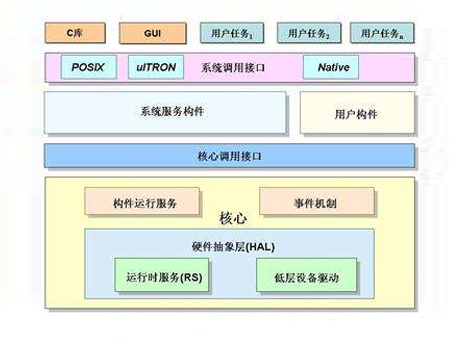
\includegraphics[width=0.7\linewidth]{R1}
	\caption{Embedded System}
	\label{Embedded System}
	\end{figure}

	\subsubsection{嵌入式系统特点}
	\begin{itemize}
	\item  \textbf{专用性强}
	
	嵌入式CPU一般是工作在特定用户群设计的系统中,具有功耗低、小体积、成本低、高集成度等特性。能够把通用CPU中由板卡完成的任务集成在芯片的内部,有利于嵌入式系统设计趋于小型化、专业化,也能够使移动功能大大增强,与网络的耦合性也大大增强。嵌入式系统有自己独立的个性化,软硬件系统的结合是非常紧密的。
	
	\item \textbf{高效率的设计}
	
	嵌入式系统的硬件和软件都必需是高效率的设计,在保证稳定、安全、可靠的基础上量体裁衣,去除冗余,争取在特定的条件和同样硅片面积下实现更高的性能,如此才能在具体应用中对处理器的选择更具有竞争力。
	
	\item \textbf{系统内核小}
	
	嵌入式系统是将半导体技术、计算机技术与电子技术和各行各业的具体应用相结合后的产物,这些结合的特性就决定了嵌入式是一个技术密集、高度分散、不断创新的知识集成系统,嵌入式系统一般是应用于小型的电子装置,系统资源相对来讲也是有限的,因此内核较传统的操作系统要小很多。
	
	\item \textbf{系统高实时性和精简}
	
	嵌入式系统中的应用软件和一般系统软件区分不明显,这样既利于控制成本,又利于实现系统安全。这是嵌入式软件的基本要求,并且软件要求固态存储,以此提高速度。而软件代码要求高可靠性、高质量和实时性。
	
	\item \textbf{有效性和创新性}
	
	嵌入式系统和具体应用有机地结合在一起,它更新换代也是和具体产品同时进行,所以嵌入式系统一旦进入市场就具有较长的生命周期,为了提升系统可靠性和执行速度,嵌入式系统中的软件一般都固化在微处理器或存储器芯片中,而不是存储在磁盘或其他载体中。
	
	\item \textbf{不具备自举开发能力}  
	
	嵌入式系统本身不具备自举开发能力。即使设计完成之后,用户通常也不能对其中的应用程序进行修改,必须有一套交叉开发工具和环境才能进行开发。
	\end{itemize}

	\subsubsection{嵌入式系统的发展趋势}
	\begin{itemize}
		
	\item 定制化
	
	嵌入式操作系统将面向特定应用提供简化型系统调用接口,专门支持一种或一类嵌入式应用。嵌入式操作系统同将具备可伸缩性、可裁减的系统体系结构,提供多层次的系统体系结构。嵌入式操作系统将包含各种即插即用的设备驱动接口。
	
	\item 精简化
	
	嵌入式操作系统继续精简系统内核,采用微内核技术,只保留和系统功能最紧密相关的软硬件,实现小尺寸、微功耗、低成本以支持小型电子设备,利用最低的资源实现最适当的功能。同时,提高产品的可靠性和可维护性。嵌入式操作系统将形成最小内核处理集,减小系统开销,提高运行效率,并可用于各种非计算机设备。这就要求设计者选用最佳的编程模型和不断改进算法,优化编译器性能,既要有丰富的硬件知识,有需要发展先进嵌入式软件技术。
	
	\item 人性化
	
	嵌入式操作系统将提供精巧的多媒体人机界面,以满足不断提高的用户需求。
	
	\item 安全化
	
	嵌入式操作系统应能够提供安全保障机制,源码的可靠性越来越高。
	
	\item 网络化
	
	面向网络、面向特定应用,嵌入式操作系统要求配备标准的网络通信接口。嵌入式操作系统的开发将越来越易于移植和联网。嵌入式操作系统将具有网络接入功能,提供TCP/UDP/IP/PPP协议支持及统一的 MAC 访问层接口,为各种移动计算设备预留接口。还有的嵌入式支持IEEE1394、USB、CAN、Bluetooth或IrDA通信接口中的一种或者几种,同时也需要提供相应的通信组网协议软件和物理层驱动软件。软件方面系统内核支持网络模块,甚至可以在设备上嵌入Web游览器,真正实现随时随地用各种设备上网。
	
	\item 标准化
	
	随着嵌入式操作系统的广泛应用的发展,信息交换、资源共享机会增多等问题的出现,需要建立相应的标准去规范其应用。
	
	\item 系统化
	
	嵌入式开发是一项系统工程,因此要求嵌入式系统厂商不仅要提供嵌入式软硬件系统本身,同时还需要提供强大的硬件开发工具和软件包支持。目前很多厂商已经充分考虑到这一点,在主推系统的同时,将开发环境也作为重点推广。比如三星在推广Arm7,Arm9芯片的同时还提供开发板和版及支持包(BSP),而WindowCE在主推系统时也提供Embedded VC++作为开发工具,还有Vxworks的Tonado开发环境,DeltaOS的Limda编译环境等等都是这一趋势的典型体现。当然,这也是市场竞争的结果。
	
	\item 功能复杂化
	
	网络化、信息化的要求随着因特网技术的成熟、带宽的提高日益提高,使得以往单一功能的设备如电话、手机、冰箱、微波炉等功能不再单一,结构更加复杂。
	
	这就要求芯片设计厂商在芯片上集成更多的功能,为了满足应用功能的升级,设计师们一方面采用更强大的嵌入式处理器如32位、64位RISC芯片或信号处理器DSP增强处理能力,同时增加功能接口,如USB,扩展总线类型,如CAN BUS,加强对多媒体、图形等的处理,逐步实施片上系统(SOC)的概念。软件方面采用实时多任务编程技术和交叉开发工具技术来控制功能复杂性,简化应用程序设计、保障软件质量和缩短开发周期。
	\end{itemize}

	\subsubsection{嵌入式系统的脆弱性}
	\begin{itemize}
		\item 供电与计算能力有限
		
		因为成本和能耗等方面的考量,嵌入式系统往往采用电池供电,且供电能力低下,基于节约系统能耗的考虑,往往无法加入过重的安全加密算法。这也导致嵌入式系统CPU的计算能力极其有限,在嵌入式系统中无法安装传统计算机上使用的杀毒软件、入侵检测系统等。同时,也无法使用传统的密码体制对其软件系统进行严格的完整性验证。恶意用户可以通过相关工具和软件,对嵌入式设备中的固件重新编程,修改成带有恶意代码或其他非法目的的固件。这给嵌入式设备带来了极大的安全隐患。
		
		\item 物理暴露
		
		很多嵌入式设备放置在远离所有者的地方,导致非法用户很容易物理接触到设备,从而对设备的软硬件进行非法的修改。如,黑客可以通过硬件搭线、探针等方式,非法刺探到系统总线,对总线中的通讯数据进行分析,或直接替换硬件系统关键部件达到绕过或者破坏原系统功能的目的。另外,存储在嵌入式设备中的非易失性数据极易被非法访问。如:恶意用户能够简单的将其中的存储芯片焊下来,通过编程器读出里面的隐私数据。
		
		\item 部署位置复杂
		
		很多嵌入式设备作为数据采集产品部署在野外等人迹罕至、条件恶劣的地方,就算发现了安全问题,维护人员也很难对其软件系统进行及时的补丁和安全升级。
		
		\item 网络接入方式多样
		
		很多的嵌入式设备具备联网的功能,其通过互联网进行数据通讯,这就进一步导致恶意用户能够在互联网的任何地方发起对设备的攻击。更为严重的是,由于嵌入式系统在设计之初,并没有考虑到这些威胁,对网络协议栈的设计考虑过于简单,很多设备在对外通讯时采用明文或只是简单加密后即通过网络发往外部,导致其极易遭受网络入侵攻击。
	\end{itemize}
	
	\subsubsection{嵌入式系统面临的(软件)安全问题}
	安全问题包含硬件问题和软件问题,但是由于我们在上OS课程,所以先掠过硬件的部分不讲。
	
	相对于硬件攻击,软件攻击的实施成本更加低廉,由于嵌入式系统需要由软件来实现相应的控制逻辑,而软件系统由于其自身固有的复杂特性,拥有更大的攻击面,成为近年来黑客主要的攻击目标。嵌入式软件系统面临诸多攻击威胁,根据不同的攻击目的,可以将这些攻击细分为篡改(以修改代码完整性为目标)、破坏(通过对运行的软件发起攻击)和窃取(以获取机密数据或隐私为目标)。
	
	\begin{itemize}
	\item 代码完整性攻击
	
	这种攻击试图修改嵌入式系统相关数据或代码。防范这类攻击的重点是保证嵌入式系统自身代码的完整性,可以在运行前通过对嵌入式系统相关代码进行安全度量,检测代码是否被篡改。Kirovski等和Chen等在系统启动之时,通过完整性传递规则,确保上层程序功能模块完整不受篡改。这些方案能够确保嵌入式软件在启动之初的静态安全性,但是缺乏针对动态安全的保护。AEGIS和OASIS架构在处理器中扩展执行完整性校验的指令集,在软件运行过程中对软件指令块和重要数据块进行完整性验证。该方案能够保护嵌入式系统运行过程中的动态完整性,但是这些方案需要对处理器进行较大改动,无法利用现有嵌入式多核处理器架构,可行性和通用性存在不足。
	
	\item 应用软件攻击
	
	针对嵌入式系统运行软件的攻击:如病毒,木马,蠕虫等通过软件代理对终端系统结构的薄弱环节发起的攻击。这类攻击是耗费代价较小,较为常见的一种形式。
	
	2016年8月,苹果公司公布了iOS下的一个高危“零日”漏洞。受害者只要点击攻击者发来的链接,手机就会被远程注入代码,攻击者瞬间就能获得受害者手机的最高权限。利用最高权限,攻击者可以远程对受害者的手机进行任何操作。这是迄今为止,苹果iOS爆出的最为危险的一个漏洞。
	
	\item 隐私数据窃取攻击
	
	这种攻击的目的是获取嵌入式系统内存储、传递或操作的敏感信息数据;防范这类攻击的主要手段是对敏感信息数据进行加密保护,但实现加密保护需要密钥,密钥的创建、存储、使用和销毁等,需要引入能够信任的密钥管理机制以保障其安全性。此外,还可通过访问控制对敏感信息数据进行保护。德国达姆施塔特工业大学的Bugiel等针对嵌入式设备中安全数据的访问和控制问题,构建TrustDroid架构,该架构在中间件层、内核层分别使用访问限制、强制访问策略,保证嵌入式关键数据的安全。
	\end{itemize}
	
	针对软件层的安全防护,常用的对策是借鉴虚拟化(VMM)技术,不需要额外的硬件开销就可以提供隔离的执行环境,让安全敏感的软件能够移植到VMM的环境中,并受保护地运行。然而,这种方案中嵌入式虚拟机监控器自身的安全性并未得到有效保障,所以受其容器管理的软件安全性实现方法也有待改进。
	
	在与软件实现相关的网络层,传统的嵌入式软件在设计之初,并没有考虑网络连接带来的安全问题。多数嵌入式硬件,都使用了TCPI/IP连接协议。基于前文的脆弱性分析,嵌入式软件在网络通讯设计中往往采用明文方式连接,软件本身并不会对通讯的数据进行任何的加密。同时,设备的身份认证全靠简单的用户名和密码机制实现,由于数据的明文传输特性,这些密码极易被攻击者捕获和破解。基于上述原因,嵌入式设备在网络接入时极易受到身份仿冒攻击;同时,在由嵌入式设备组成的内部网络中,节点也极易遭受间谍和木马的攻击,节点之间的数据也会被攻击者进行截获、篡改和伪造。
	
	\subsubsection{嵌入式系统安全对策(软件)}
	针对嵌入式软件系统的安全对策,现有的安全解决方案,从虚拟化、操作系统、应用层和网络传输层几个方面,通过资源隔离、安全审计、应用防护和轻量加密方案的角度对其进行安全加固。
	
	\begin{itemize}
	
	\item 基于虚拟化的安全对策
	
	有研究者通过借鉴传统x86架构的虚拟化技术,对相关资源进行隔离和虚拟化以达到安全增强的目的。有通过在操作系统层引入虚拟化机制,并建立可信安全实体,对用户态的进程进行隔离。该安全实体控制和管理Android系统中的进程,并提供对设备中的软件进行远程监管的接口。有将Linux的容器组件移植到Android系统,通过隔离容器,在系统内核之上建立多个虚拟的Android框架,以达到各App之间安全隔离的目的。尽管这些虚拟化技术能够通过隔离思想来解决上层的安全问题,但在虚拟化架构之下,缺乏安全的根基,无法保障虚拟化架构自身的安全。
	
	\item 操作系统层安全对策
	
	近年来,很多研究者基于系统挂钩(hooks)的思想来对系统进行安全增强。有提出了一种“Android安全模型框架”(Android security modules,ASM),利用系统挂钩构建相关监控模块,达到Android系统安全性增强的目的。有从策略控制的角度,提出了一种称为DeepDroid的企业级安全策略增强机制。该机制通过动态实施一个细粒度的系统级服务,让管理员能够对系统资源访问策略进行控制。DroidForce和WrapDroid也基于同样的思想,利用对系统策略进行相应的控制和强化来提高安全级别。但是基于同样的原因,无论是系统挂钩还是安全策略,都没有底层的机制对自身进行保护,其安全架构是不完善的。
	
	\item 应用软件层安全对策
	
	也有研究人员站在安全审查的角度,提出了安全增强的相关方案。有设计并实现了一款Dex文件的比较工具Dexdiff,对已经编译好的Android二进制文件进行结构化的比较,并能给出上下文的差异。从而通过应用级的比较与审查,找出潜在的恶意应用。基于类似的设计思想,TaintDroid与PiOS通过动态污点跟踪与静态数据流分析的方法,能审计出应用程序可能存在的隐私泄露。还有研究人员聚焦于恶意软件检测,通过各种手段对软件进行检查,找出恶意的应用。虽然上述这些方法能够有效地对应用程序进行审查,但对于应用层之下的安全,却无能为力。
	
	\item 网络传输层安全对策
	
	为了解决网络的明文传输问题,同时又兼顾嵌入式硬件功耗和计算能力有限的特点,有研究者设计了专门针对嵌入式设备的轻量级加密方案。为了解决身份仿冒的问题,一般的安全增强方法,是在设备的生产过程中,为每一个设备生成唯一的ID,分别存储在设备和远端的数据库中。
	
	\end{itemize}
	虽然上述方法能够有效地避免明文传输和身份仿冒问题,但身份标识和密钥往往用明文或简单的编码方式存储在设备中,缺乏一体化的保护措施。一旦攻击者能够物理接触到设备,整个网络的身份认证和数据传输保护便形同虚设。	
	
	\subsection {用Rust编写嵌入式操作系统的优势}
	\begin{itemize}
	\item 运行时库
	
	编程语言的运行时库,通常理解为,其编译出的可执行程序在运行时必须依赖的非操作系统本身的动态库。例如 C 程序必须依赖 msvcrt 或 glibc,Java 程序必须依赖 JRE,VB 程序必须依赖 msvbvm,易语言程序必须依赖 krnln.fne/fnr,等等。由于 C 运行时库往往跟操作系统紧密集成(尤其是类 Unix 系统),可以认为 C 运行时库是操作系统的一部分,进而认为 C 没有运行时库(有争议)。如果认同这一点,那么,经过静态编译生成的 Rust 程序,运行时仅依赖 C 运行时库,也就可以认为没有运行时库了。即使不认同这一点,等以后 Rust 支持了静态链接 MUSL 库(同时抛弃掉 glibc),依然能够做到没有运行时库。当然,动态编译的 Rust 程序中运行时还是必须依赖标准库 libstd-\\*.so 等动态库的,这是给予程序员的额外可选项。
	
	没有运行时库的优势在于,运行时库本身也具有平台依赖性或运行时依赖性,没有运行时库,则程序的所有代码都是程序员可控的。
	
	\item 运行时损耗
	
	程序的运行时损耗,是指程序在运行过程中所必须付出的额外的代价。例如 Java 的虚拟机、C\# 的垃圾回收器、脚本语言的解释器等等,这些子系统本身在运行时都会消耗数量可观的内存和 CPU,影响程序和系统的运行性能。而 Rust 没有虚拟机、垃圾回收器和解释器,所以没有这类运行时损耗。
	
	此外,内存管理、栈管理、调用操作系统 API 和 C 库等各种情况下,都有可能产生额外的运行时损耗。
	
	Rust 运行时需要每个函数执行 morestack 检查栈溢出(morestack 已被取消),为了内存安全这是“必需的”检查,而以 C 语言的思路去看可能就是“额外的”损耗,无论如何这项运行时损耗很小。Unwinding 仅发生在 panic 之后,不视为运行时损耗。Rust 采用 jemalloc 管理内存(也可禁用),不仅没有运行时损耗,反而带来运行效率的明显提升。
	
	Rust 的 Rc 类型以引用计数管理对象内存,Arc 类型以 Atomic 引用计数管理对象内存,这是较小的运行时损耗。但如果程序员不主动使用 Rc/Arc 类型,则无需为此付出额外的代价。
	
	Go 语言的协程调度器,当然也有运行时损耗,但这在某种程度上是程序实现自身功能的必要,算不上“额外的”代价,如果不需要此功能则损耗很小,故本文作者不视其为运行时损耗。而其通过 channel 共享内存、管理逐步连续增长的栈、调用 C 库和系统 API,则被视为运行时损耗,因为这些都是“非必要的”损耗,而且损耗还不小。
	
	那 Java 的 JIT 编译器在运行时把字节码编译为机器码,算不算运行时损耗呢?损耗肯定是有的,但仅在特定条件下触发,且其带来的收益可能远大于损耗,是提升运行性能的必要步骤,故不认为它引入了“额外的”代价,不视其为运行时损耗。而 Java 的虚拟机和垃圾收集器,显然是突出的运行时损耗。
	
	\item 核心库
	
	Rust 核心库,可以理解为是经过大幅精简的标准库,它被应用在标准库不能覆盖到的某些少数特定领域,如嵌入式开发。
	
	核心库不依赖任何操作系统,也不提供文件 / 网络 / 多线程 / 内存申请释放相关的任何功能,因而可移植性更好、应用范围更广。
	
	在代码开头写上 \textbf{\# ! [no\_std] }就代表放弃标准库,而使用核心库。
	
	核心库里面有:基础的接口性数据类型(参见上文,下同)、基础类型操作接口、常用的功能性数据类型、常用的宏定义、底层操作接口等,而且跟标准库 API 几乎是完全一致的;再配合 alloc 库(或自己定制的 alloc 库)又有了内存申请释放功能;再加上 collections 库,String/Vec/HashMap 等也有了。事实上从内部实现来说,标准库里的某些功能正是来源于核心库(以及 alloc/collections 等)。
	
	\item 内存安全
	
	内存不安全的后果十分严重,“心脏出血”漏洞(Heartbleed)重创全球IT行业。其源于OpenSSL【越界访问内存】。OS/GLIBC/JAVA/浏览器等频繁爆出重大安全漏洞,多数都与错误使用内存有关。
	
	传统C/C++语言放弃解决内存安全问题,程序员因疏忽或犯错很容易制造内存安全漏洞。使用GC能基本保证内存安全,但牺牲了运行时性能。
	
	Rust针对内存安全做了严格的限制。\\
	安全地读写内存\\
	• 在限定时间和空间范围内读写内存\\
	• 防止被他人意外修改或释放\\
	• 避免访问空指针和野指针\\
	安全地释放内存\\
	• 在恰当的时机释放\\
	• 确保释放,不遗漏\\
	• 仅释放一次\\
	而C语言中可能产生指针越界,野指针,NULL指针解引用,并发读写导致数据竞争,缓冲区溢出,段错误等各种危险操作。
	
	总体来说Rust语言具有很强的控制性和很高的安全性,且运行效率高,无GC无VM。
	\end{itemize}


	\section{相关工作}
	\subsection{学术界相关工作调研}
	因为其安全性及运行效率这两大得天独厚的优势,Rust语言从诞生之日起就一直有取代C语言在系统编程中的地位的趋势。Rust社区也一直在努力使从经典的C代码向Rust代码进行迁移的过程更加方便快捷。\textbf{C2Rust}就是其中一个重要的尝试,它通过一个基于Clang的C到Rust翻译器将C语言代码完全按语义翻译成不安全的(unsafe) Rust,为程序员进一步重构或重写代码提供了方便。同时,它还提供了测试C代码和Rust代码功能一致性的工具。但是,其翻译出的代码存在可读性不高的问题,因此,我们在本课题中不会使用该工具。
	
\begin{figure}[H]
	\centering
	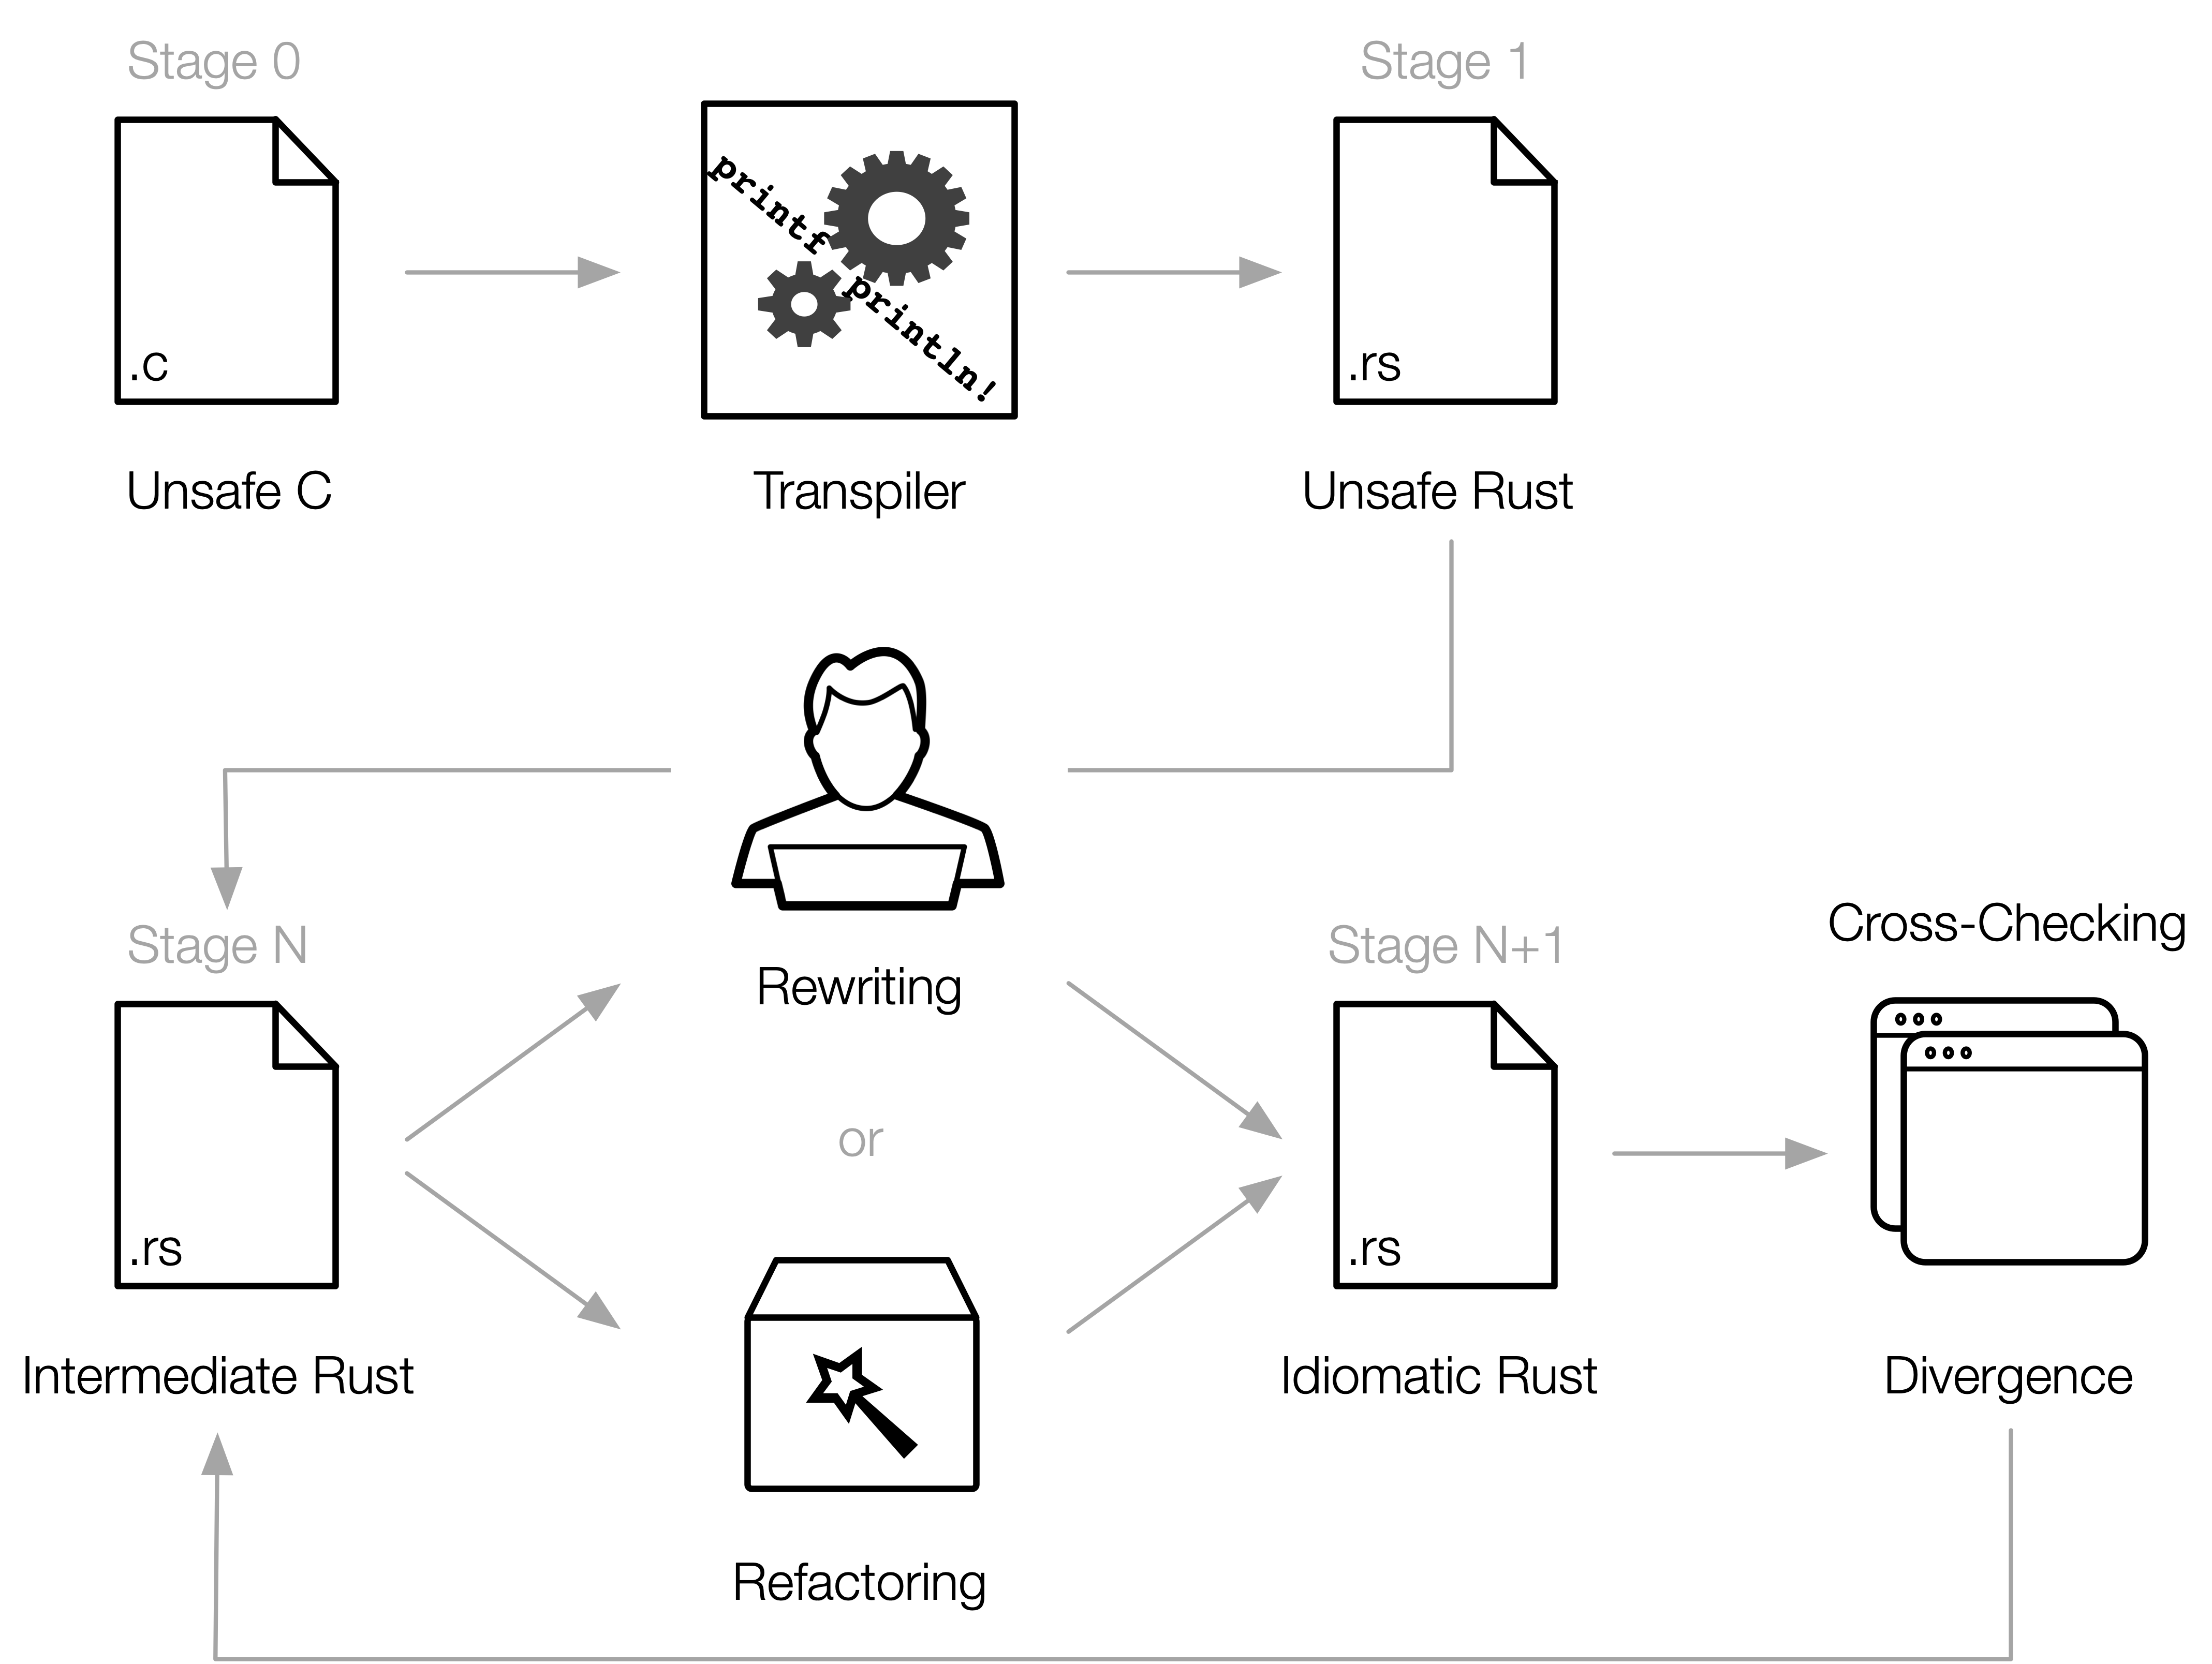
\includegraphics[width=1.0\linewidth]{c2rust-overview}
	\caption{c2rust-overview}
	\label{fig:c2rust-overview}
\end{figure}
	
	\textbf{freertos.rs}是和我们最为相似的一个项目,它提供了FreeRTOS系统API的Rust语言封装,它通过在Rust代码中嵌入形如"extern C"的C语言调用来和FreeRTOS的API进行通信,因此它目前还会使用C语言的动态内存分配,这可能存在内存安全隐患。
	
	\textbf{Redox}是一个用Rust语言编写的类UNIX操作系统 , 它的目标是把Rust语言带来的创新引入到一个现代的微内核和全系列的应用程序。与实时操作系统不同的是,它实现了现代操作系统的大多特性,包括图形界面、设备驱动器等。
	
	\textbf{Mozilla}一直以来是Rust语言最重要的支持者,他们已经在其许多产品开发中使用Rust编程,其中包括Servo和Firefox浏览器内核的一些重要成分。自Firefox 54以来,Firefox的所有平台都需要Rust支持,在Firefox 56和57中出现了主要由Rust编写的部件。
	
	在2018年的OSH课程中,Rocker团队利用Rust改写了FreeRTOS的7.1.0版本中涉及任务管理的几个函数。他们的工作是我们本次课题的参考,但他们因为采用了Rust语言和C语言混合编程的方式,导致在开发的过程中遇到了很大的困难,此外,这种代码编写方式也不能充分地利用Rust的安全性。
	
	此外,coreutil是利用Rust重写的GNU coreutil实现,xsv是利用Rust编写的快速CSV处理工具。他们都利用了Rust语言的跨平台性和稳定性的特点。
	\subsection{工业界相关工作调研}
	\textbf{Rust因其内存管理的安全性和高效性,在近两年内飞速发展,建立起了完善的开发人员社区,在工业界也大展拳脚,在多个领域催生出了安全高效的虚拟产品。}
	\subsubsection{Rust in Optimization——npm堆栈管理}
		
		
		npm是Node.js的包管理工具。得益于强大的功能,npm注册表成为世界上最大的软件注册表。但在规模成指数增长的同时,npm同样面临诸多挑战,其中一个是扩展CPU绑定服务(CPU-bound Service)产生的性能瓶颈:npm执行的大多数操作都是网络绑定的,JavaScript能够较好地支持该功能,但是在检查是否允许用户发布包的授权服务时,npm团队发现JS在执行一些CPU绑定任务时会造成性能下降。因此Node.js中这一服务需要重新实现,而npm团队希望借此机会利用Rust代码来提高性能。
		\begin{figure}[H]
			\centering
			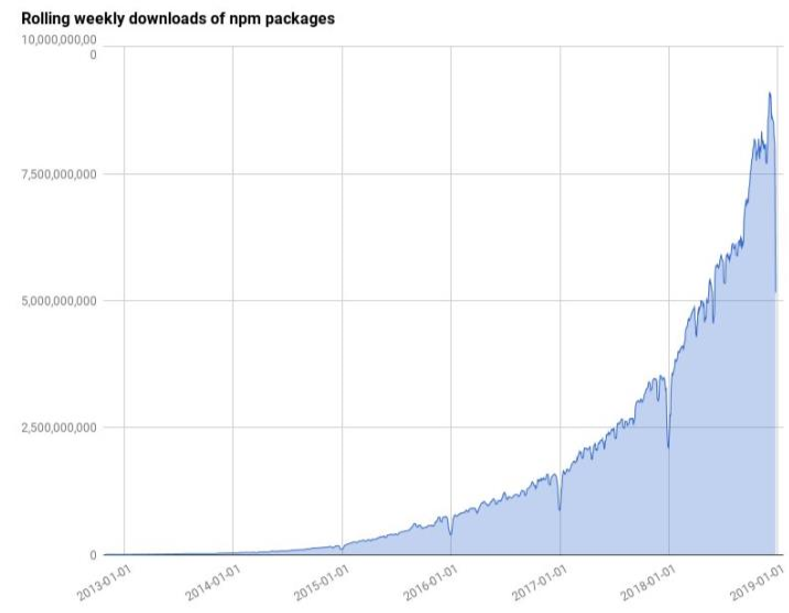
\includegraphics[width=0.7\linewidth]{Z1}
			\caption{NPM}
			\label{fig:southeast}
		\end{figure}
		C或C ++解决方案不再是一个合理的选择。这些语言需要内存管理方面的专业知识,以免出现安全问题,崩溃和内存泄漏(事实上,有专业知识的程序员也难免在百万行代码中犯一些这样的错误)。而Java由于需要将JVM和相关库部署在服务器上,这将产生一系列资源开销,不利于性能的提升。
		Rust代码实现的优势:
		\begin{itemize} 
		\item 内存安全
		\item 编译为独立且易于部署的二进制文件
		\item 总是优于JavaScript
		\end{itemize}
		它是一种可扩展且易于部署的解决方案,可以降低资源使用率而不会影响内存安全性。Cargo的依赖管理为系统编程领域带来了现代工具,它独立地为每个项目协调每个依赖项的版本,以便环境中的构建项目不会影响最终的可执行文件。npm的第一个Rust程序在一年半的应用过程中没有引起任何警报。
		
		不过npm团队坦言:在Rust中重写服务确实需要比JavaScript版本和Go版本更长的时间,需要大约一周的时间来熟悉语言并实现程序。 Rust语言的设计预先加载了关于内存使用的决策,以确保内存的安全性。

		\subsubsection{Rust in Analysis——Skylight代理的优化}
		Tilde是一家位于波特兰的创业公司,他们开发的产品Skylight能够将Ruby on Rails框架中应用程序的性能数据转化为易于分析的信息,以便开发人员高效地监控和维护应用程序。Skylight代理在客户开发的rails应用程序中运行,以监控实际性能指标。但用户对这款软件的分析性能要求比较高:第一,他们对此代理使用的内存和CPU开销的容差非常低。由于这款代理用于帮助开发人员分析程序为什么变慢,因此很重要的一点是代理本身不会对应用程序的性能产生影响。第二,大多数Skylight的客户在Heroku上托管他们的应用程序,他们受到256或512 MB内存限制。
		
		在先前的Ruby版本中,Skylight的内存使用量经常超过100MB,此时Heroku会报出内存超过限制的错误并重启代理。
		\begin{figure}[H]
			\centering
			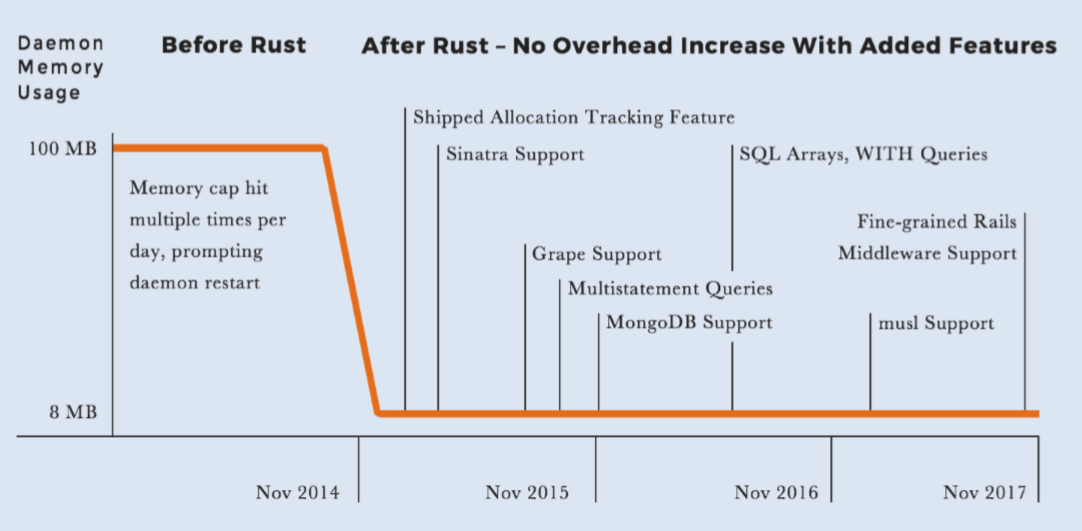
\includegraphics[width=0.7\linewidth]{Z2}
			\caption{Skylight}
			\label{fig:southeast2}
		\end{figure}
		而在使用Rus替换Ruby的数据结构并重写代理后,Skylight的内存占用能够保持在8 MB,比Ruby减少了92%,极大地减小了内存开销。
		
		除此之外,Rust在编译时避免了数据竞争的问题。在一个Rust工程师希望使用新的数据结构来优化日志功能、防止消息重复时,Rust编译器报了错,表明这个数据结构中的某一部分不能很好地发挥系统中固有的并发性。修复后,应用程序就能够稳定实现预期的功能。Rust能够在早期开发过程中捕获并提醒程序员解决此类问题。
		
		\subsubsection{Rust in Entertainment——大型游戏安全流畅的并发性}
		目前许多游戏都是用C++编写的。无论是2D还是3D,大型游戏都有许多大型数据结构来保存游戏渲染图形所需的大量信息。游戏需要缓存这些数据以便快速访问,同时还需要经常更改数据以便响应。如果使用C#或Java等垃圾收集语言(garbage-collection language)编写,那么游戏体验会受到游戏截图等停顿的明显影响。
		
		Chucklefish团队使用Rust创建了一个利用多个核心而不会崩溃的游戏。他们仍编写了一些额外代码来确保组件和资源的锁定不会与其他系统发生死锁,Rust编译器会在出现这样的潜在风险时发出警告。开发人员不必在处理数据竞争的问题上小心翼翼,可以将之间花在处理游戏的运行逻辑上。
		
		Rust还能够很好地处理跨平台差异。在开发Xbox、S4和Nintendo Switch等不同的主机适用版本时,Rust的包管理器工具Cargo为Chucklefish的构建处理了依赖库的问题。而在过去,添加一个库就需要花费数天的时间才能成功集成到所有支持的平台上。除此之外,Chucklefish开发人员认为,Rust中的类型和API需要更少的自定义包装代码,使用起来也更加自然。
		
	\section{Rust调研}
	\subsection{越来越多的用户体会到Rust语言的高效性}
	
\begin{figure}[H]
	\centering
	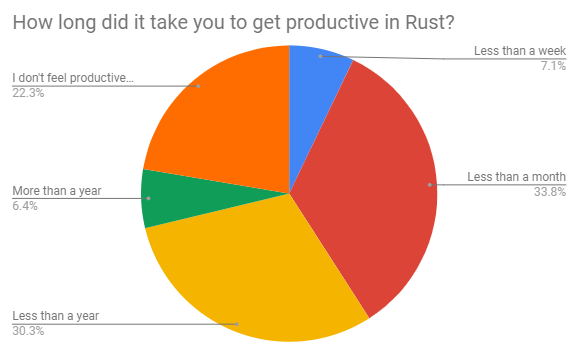
\includegraphics[width=0.7\linewidth]{n1}
	\caption{Rust1}
	\label{fig:n1}
\end{figure}
	超过40\%的Rust用户在不到一个月的使用内即感受到Rust语言的高效性,超过70\%的用户在不到一年内感受到Rust语言的高效性。   
	\subsection{Rust使用规模增大}
	
\begin{figure}[H]
	\centering
	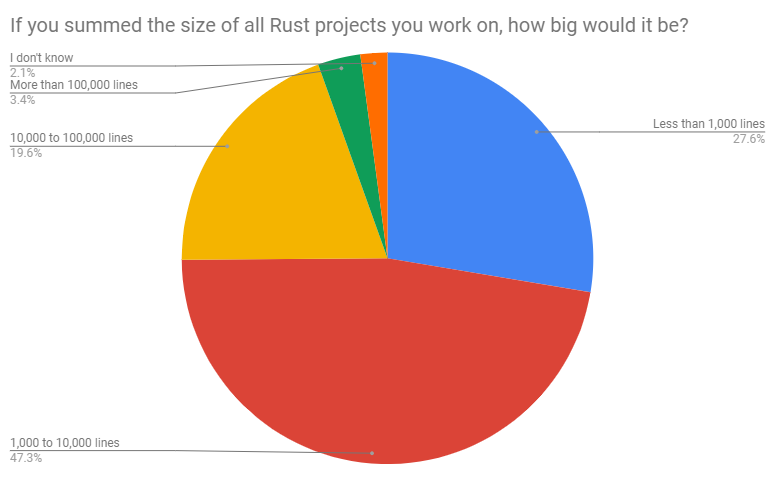
\includegraphics[width=0.7\linewidth]{n2}
	\caption{Rust 2}
	\label{fig:n2}
\end{figure}
2018年,调查显示,约23%的Rust用户使用Rust编写了超过10k行代码,超过70%用户使用Rust编写超过1k行代码。   
此外,随着对Rust项目的整体投资增加,Rust项目将趋向更大规模。Rust的中大型投资(分别超过10k和10万行代码)从2016年的8.9%增长到2017年的16%,2018年增长到23%。    
	\subsection{使用Rust的目标平台趋于多样化}
	
\begin{figure}[H]
	\centering
	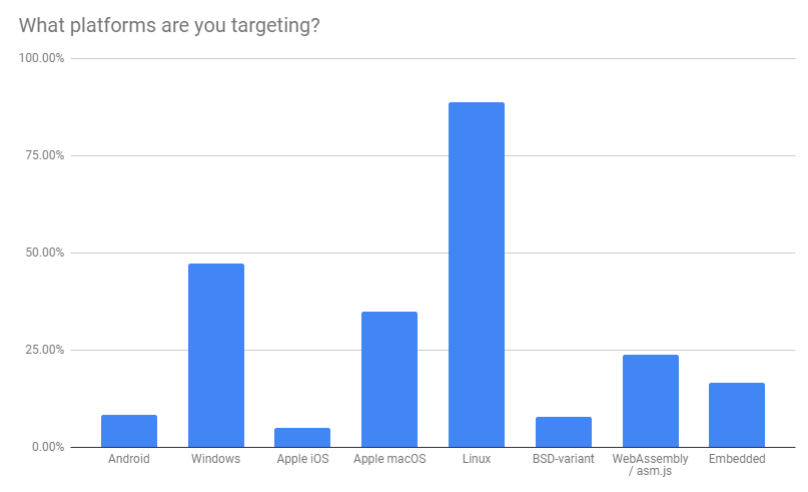
\includegraphics[width=0.7\linewidth]{n3}
	\caption{Rust 3}
	\label{fig:n3}
\end{figure}
	Linux和Windows为Rust语言的主要目标平台。但在2017年,针对移动端、嵌入式设备的Rust开发大幅增长,交叉编译大大增加。2018年,针对WebAssembly的开发大幅增加,较2017年几乎翻了一番。
	
	\subsection{人们对Rust语言的兴趣与日俱增}
	
\begin{figure}[H]
	\centering
	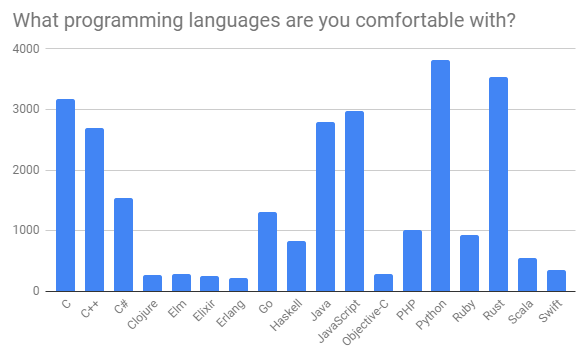
\includegraphics[width=0.7\linewidth]{n4}
	\caption{Rust 4}
	\label{fig:n4}
\end{figure}
	自2016年开始,Rust连续三年成为Stack Overflow开发者调查中“最受欢迎的编程语言” 。同时,根据Rust官网进行的用户调查,2018年,Rust成为用户熟悉的编程语言第二名,仅次于python。
	
	\subsubsection{目前已使用Rust开发的项目}
	使用Rust开发的项目日益增加,目前已使用Rust开发的项目主要集中于浏览器、操作系统等.   
	\begin{itemize}
		\item 浏览器:
		\subitem 并行网页浏览器引擎Servo
		\subitem 用于改进Firefox的Gecko Web浏览器引擎Quantum 
		\item 操作系统:
		\subitem Magic Pocket –  Dropbox的文件系统,为Diskotech PB级存储设备提供动力      
		\subitem Redox – 微内核操作系统   
		\subitem Stratis – 用于Fedora 28的文件系统   
		\subitem Railcar – Oracle的一个容器的运行时    
		\subitem Firecracker – 针对无服务器计算的安全、快速的微型虚拟机   
	\end{itemize}
	
	\subsubsection{Rust目前的挑战}
	Rust语言目前虽然稳步发展,吸引了更多的用户,应用场景更加广泛,但仍存在许多挑战。根据Rust官网2018年的调查结果,有以下地方仍待改进:需要更好的函数库、更好的IDE、更丰富的工具、改进编译时间等。   
	
	\subsubsection{Rust用于嵌入式设备开发的优势}
	\begin{itemize}
		\item 强大的静态分析:Rust将在在编译时强制执行引脚和外设配置,以保证程序非预期部分不会使用资源。   
		\item 灵活的内存管理:可选择动态内存分配、全局分配和动态数据结构,或省略堆全部进行静态分配。
		\item 无畏并发:Rust保证线程间不会意外共享状态,可以使用任何并行方式。   
		\item 互通性:可将Rust集成到已编写的C代码库中,或使用现有SDK编写Rust应用。
		\item 可移植性:编写一次库或驱动,即可应用于各类系统中。
	\end{itemize}
	
	\section{FreeRTOS调研}
	\subsection{FreeRTOS v10.2.0 task.c 中任务创建API}
\subsubsection {xTaskCreate}

\begin{lstlisting}[language={[ANSI]C},keywordstyle=\color{blue!70},commentstyle=\color{red!50!green!50!blue!50},frame=shadowbox, rulesepcolor=\color{red!20!green!20!blue!20}]
BaseType_t xTaskCreate(TaskFunction_t pvTaskCode,
                       const char * const pcName,
                       configSTACK_DEPTH_TYPE usStackDepth,
                       void *pvParameters,
                       UBaseType_t uxPriority,
                       TaskHandle_t *pvCreatedTask);
\end{lstlisting}

创建一个任务,并且自动为其分配\textbf{栈空间}和\textbf{数据空间}。

\subsubsection {xTaskCreateStatic}

\begin{lstlisting}[language={[ANSI]C},keywordstyle=\color{blue!70},commentstyle=\color{red!50!green!50!blue!50},frame=shadowbox, rulesepcolor=\color{red!20!green!20!blue!20}]
TaskHandle_t xTaskCreateStatic( TaskFunction_t pvTaskCode,
				const char * const pcName,
				uint32_t ulStackDepth,
				void *pvParameters,
				UBaseType_t uxPriority,
				StackType_t *pxStackBuffer,
				StaticTask_t *pxTaskBuffer );
\end{lstlisting}
创建一个任务,此时需要程序员来提供一个\textbf{栈空间}和\textbf{数据空间}的地址。

\subsubsection {xTaskCreateRestricted}
\begin{lstlisting}[language={[ANSI]C},keywordstyle=\color{blue!70},commentstyle=\color{red!50!green!50!blue!50},frame=shadowbox, rulesepcolor=\color{red!20!green!20!blue!20}]
BaseType_t xTaskCreateRestricted(TaskParameters_t  *pxTaskDefinition,
				TaskHandle_t *pxCreatedTask );
\end{lstlisting}

创建一个任务,此时需要程序员手动提供一个\textbf{栈空间}地址。

\subsubsection {xTaskCreateRestrictedStatic}

\begin{lstlisting}[language={[ANSI]C},keywordstyle=\color{blue!70},commentstyle=\color{red!50!green!50!blue!50},frame=shadowbox, rulesepcolor=\color{red!20!green!20!blue!20}]
 BaseType_t xTaskCreateRestrictedStatic( 
 			TaskParameters_t *pxTaskDefinition, 
 			TaskHandle_t *pxCreatedTask );
\end{lstlisting}

创建一个任务,需要程序员手动提供\textbf{栈空间}地址。\textbf{数据空间}会被自动地动态分配。

\subsubsection {vTaskAllocateMPURegions}

\begin{lstlisting}[language={[ANSI]C},keywordstyle=\color{blue!70},commentstyle=\color{red!50!green!50!blue!50},frame=shadowbox, rulesepcolor=\color{red!20!green!20!blue!20}]
void vTaskAllocateMPURegions( TaskHandle_t xTask, 
	 const MemoryRegion_t * const pxRegions );
\end{lstlisting}

用来为\textbf{restricted task}分配内存空间。

\subsubsection {vTaskDelete}

\begin{lstlisting}[language={[ANSI]C},keywordstyle=\color{blue!70},commentstyle=\color{red!50!green!50!blue!50},frame=shadowbox, rulesepcolor=\color{red!20!green!20!blue!20}]
void vTaskDelete( TaskHandle_t xTask );
\end{lstlisting}

删除一个任务。


\subsection {FreeRTOS v10.2.0 task.c 中任务控制API}

\subsubsection {vTaskDelay}

\begin{lstlisting}[language={[ANSI]C},keywordstyle=\color{blue!70},commentstyle=\color{red!50!green!50!blue!50},frame=shadowbox, rulesepcolor=\color{red!20!green!20!blue!20}]
void vTaskDelay( const TickType_t xTicksToDelay );
\end{lstlisting}

以给定参数来延迟任务。

\subsubsection {vTaskDelayUntil}

\begin{lstlisting}[language={[ANSI]C},keywordstyle=\color{blue!70},commentstyle=\color{red!50!green!50!blue!50},frame=shadowbox, rulesepcolor=\color{red!20!green!20!blue!20}]
void vTaskDelayUntil( TickType_t *pxPreviousWakeTime, 
		      const TickType_t xTimeIncrement );
\end{lstlisting}

指定某个确定的时间点来解除阻塞。

\subsubsection {xTaskAbortDelay}

\begin{lstlisting}[language={[ANSI]C},keywordstyle=\color{blue!70},commentstyle=\color{red!50!green!50!blue!50},frame=shadowbox, rulesepcolor=\color{red!20!green!20!blue!20}]
BaseType_t xTaskAbortDelay( TaskHandle_t xTask );
\end{lstlisting}

让任务从跳出阻塞状态回到它原来被调用的地方。

\subsubsection {uxTaskPriorityGet}

\begin{lstlisting}[language={[ANSI]C},keywordstyle=\color{blue!70},commentstyle=\color{red!50!green!50!blue!50},frame=shadowbox, rulesepcolor=\color{red!20!green!20!blue!20}]
UBaseType_t uxTaskPriorityGet( const TaskHandle_t xTask );
\end{lstlisting}

获得任务的优先级。

\subsubsection {eTaskGetState}

\begin{lstlisting}[language={[ANSI]C},keywordstyle=\color{blue!70},commentstyle=\color{red!50!green!50!blue!50},frame=shadowbox, rulesepcolor=\color{red!20!green!20!blue!20}]
eTaskState eTaskGetState( TaskHandle_t xTask );
\end{lstlisting}

获取任务的状态码,是一个枚举类型。

\subsubsection {vTaskGetInfo}

\begin{lstlisting}[language={[ANSI]C},keywordstyle=\color{blue!70},commentstyle=\color{red!50!green!50!blue!50},frame=shadowbox, rulesepcolor=\color{red!20!green!20!blue!20}]
void vTaskGetInfo( TaskHandle_t xTask, 
		   TaskStatus_t *pxTaskStatus,
		   BaseType_t xGetFreeStackSpace,
		   eTaskState eState );
\end{lstlisting}

获取任务的信息。

\subsubsection {vTaskPrioritySet}

\begin{lstlisting}[language={[ANSI]C},keywordstyle=\color{blue!70},commentstyle=\color{red!50!green!50!blue!50},frame=shadowbox, rulesepcolor=\color{red!20!green!20!blue!20}]
void vTaskPrioritySet( TaskHandle_t xTask,
		       UBaseType_t uxNewPriority );
\end{lstlisting}

设置任务的优先级。

\subsubsection {vTaskSuspend}

\begin{lstlisting}[language={[ANSI]C},keywordstyle=\color{blue!70},commentstyle=\color{red!50!green!50!blue!50},frame=shadowbox, rulesepcolor=\color{red!20!green!20!blue!20}]
void vTaskSuspend( TaskHandle_t xTaskToSuspend );
\end{lstlisting}

挂起任务。

\subsubsection {vTaskResume}

\begin{lstlisting}[language={[ANSI]C},keywordstyle=\color{blue!70},commentstyle=\color{red!50!green!50!blue!50},frame=shadowbox, rulesepcolor=\color{red!20!green!20!blue!20}]
void vTaskResume( TaskHandle_t xTaskToResume );
\end{lstlisting}

继续执行被挂起的任务。

\subsection {FreeRTOS v10.2.0 task.c 中程序调度API}

\subsubsection {vTaskStartScheduler}

\begin{lstlisting}[language={[ANSI]C},keywordstyle=\color{blue!70},commentstyle=\color{red!50!green!50!blue!50},frame=shadowbox, rulesepcolor=\color{red!20!green!20!blue!20}]
void vTaskStartScheduler( void );
\end{lstlisting}

启动任务调度程序。

\subsubsection {vTaskEndScheduler}

\begin{lstlisting}[language={[ANSI]C},keywordstyle=\color{blue!70},commentstyle=\color{red!50!green!50!blue!50},frame=shadowbox, rulesepcolor=\color{red!20!green!20!blue!20}]
void vTaskEndScheduler( void );
\end{lstlisting}

停止任务调度程序,在处理完后,又重新从\textbf{vTaskStartScheduler}开始。

\subsubsection {vTaskSuspendAll}

\begin{lstlisting}[language={[ANSI]C},keywordstyle=\color{blue!70},commentstyle=\color{red!50!green!50!blue!50},frame=shadowbox, rulesepcolor=\color{red!20!green!20!blue!20}]
void vTaskSuspendAll( void );
\end{lstlisting}

在不终止中断的情况下挂起调度程序。

\subsubsection {xTaskResumeAll}

\begin{lstlisting}[language={[ANSI]C},keywordstyle=\color{blue!70},commentstyle=\color{red!50!green!50!blue!50},frame=shadowbox, rulesepcolor=\color{red!20!green!20!blue!20}]
BaseType_t xTaskResumeAll( void );
\end{lstlisting}

继续执行被挂起的调度程序。

\subsubsection {xTaskGetTickCount}

\begin{lstlisting}[language={[ANSI]C},keywordstyle=\color{blue!70},commentstyle=\color{red!50!green!50!blue!50},frame=shadowbox, rulesepcolor=\color{red!20!green!20!blue!20}]
TickType_t xTaskGetTickCount( void );
\end{lstlisting}

获取从`vTaskStartScheduler`被调用到现在的毫秒数。

\subsubsection {uxTaskGetNumberOfTasks}

\begin{lstlisting}[language={[ANSI]C},keywordstyle=\color{blue!70},commentstyle=\color{red!50!green!50!blue!50},frame=shadowbox, rulesepcolor=\color{red!20!green!20!blue!20}]
uint16_t uxTaskGetNumberOfTasks( void );
\end{lstlisting}

返回内核正在管理的任务的子总数目。

\subsubsection {pcTaskGetName}

\begin{lstlisting}[language={[ANSI]C},keywordstyle=\color{blue!70},commentstyle=\color{red!50!green!50!blue!50},frame=shadowbox, rulesepcolor=\color{red!20!green!20!blue!20}]
char *pcTaskGetName( TaskHandle_t xTaskToQuery );
\end{lstlisting}

返回任务的名字。

\subsubsection {xTaskGetHandle}

\begin{lstlisting}[language={[ANSI]C},keywordstyle=\color{blue!70},commentstyle=\color{red!50!green!50!blue!50},frame=shadowbox, rulesepcolor=\color{red!20!green!20!blue!20}]
TaskHandle_t xTaskGetHandle( const char *pcNameToQuery );
\end{lstlisting}

返回任务的句柄。

\subsubsection {uxTaskGetStackHighWaterMark}

\begin{lstlisting}[language={[ANSI]C},keywordstyle=\color{blue!70},commentstyle=\color{red!50!green!50!blue!50},frame=shadowbox, rulesepcolor=\color{red!20!green!20!blue!20}]
UBaseType_t uxTaskGetStackHighWaterMark( TaskHandle_t xTask );
\end{lstlisting}

返回栈使用空间最大的那次数值。

\subsubsection {xTaskCallApplicationTaskHook}

\begin{lstlisting}[language={[ANSI]C},keywordstyle=\color{blue!70},commentstyle=\color{red!50!green!50!blue!50},frame=shadowbox, rulesepcolor=\color{red!20!green!20!blue!20}]
BaseType_t xTaskCallApplicationTaskHook( TaskHandle_t xTask, 
                                         void *pvParameter );
\end{lstlisting}

执行相应的钩子函数。

\subsubsection {xTaskGetIdleTaskHandle}

\begin{lstlisting}[language={[ANSI]C},keywordstyle=\color{blue!70},commentstyle=\color{red!50!green!50!blue!50},frame=shadowbox, rulesepcolor=\color{red!20!green!20!blue!20}]
TaskHandle_t xTaskGetIdleTaskHandle( void );
\end{lstlisting}

返回空闲任务的句柄。

\subsubsection {xTaskGetIdleRunTimeCounter}

\begin{lstlisting}[language={[ANSI]C},keywordstyle=\color{blue!70},commentstyle=\color{red!50!green!50!blue!50},frame=shadowbox, rulesepcolor=\color{red!20!green!20!blue!20}]
TickType_t xTaskGetIdleRunTimeCounter( void );
\end{lstlisting}

返回空闲任务的运行时间。

\subsubsection {xTaskNotify}

\begin{lstlisting}[language={[ANSI]C},keywordstyle=\color{blue!70},commentstyle=\color{red!50!green!50!blue!50},frame=shadowbox, rulesepcolor=\color{red!20!green!20!blue!20}]
BaseType_t xTaskNotify( TaskHandle_t xTaskToNotify, 
			uint32_t ulValue, 
			eNotifyAction eAction );
\end{lstlisting}

发送广播。

\subsubsection {xTaskNotifyWait}
\begin{lstlisting}[language={[ANSI]C},keywordstyle=\color{blue!70},commentstyle=\color{red!50!green!50!blue!50},frame=shadowbox, rulesepcolor=\color{red!20!green!20!blue!20}]
BaseType_t xTaskNotifyWait( uint32_t ulBitsToClearOnEntry, 
			    uint32_t ulBitsToClearOnExit, 
                            uint32_t *pulNotificationValue, 
                            TickType_t xTicksToWait );
\end{lstlisting}

等待广播。



\subsection {queue.c文件中的重要函数}

\subsubsection {xQueueCreate}

创建一个队列。

\subsubsection {xQueueCreateStatic}

使用静态方式创建一个队列。

\subsubsection {xQueueSendToToFront}

将一个元素送到队首。

\subsubsection {xQueueSendToBack}

将一个元素送到队尾。

\subsubsection {xQueueSend}

插入一个元素到队列中。

\subsubsection {xQueueOverwrite}

插入一个元素到队列中,如果队列已经满,则覆盖。

\subsubsection {xQueueGenericSend}

和`xQueueSend`效果相同,但是是推荐的API。

\subsubsection {xQueuePeek}

获取一个队列中中的元素但是不删除其在队列中的位置。

\subsubsection {xQueueReceive}

获取一个队列中的元素,成功访问后就删除该元素在队列中的位置。

\subsubsection {uxQueueMessagesWaiting}

返回储存在队列中信息的数目。

\subsubsection {uxQueueSpacesAvailable}

返回队列中的可用空间。

\subsubsection {vQueueDelete}

删除队列。

> 上面的函数定义是为了在任务间传输数据,下面的函数用于`co-routines`(联合任务)

\subsection {list.c 中的主要函数}

\subsubsection {vListInitialise}

\begin{lstlisting}[language={[ANSI]C},keywordstyle=\color{blue!70},commentstyle=\color{red!50!green!50!blue!50},frame=shadowbox, rulesepcolor=\color{red!20!green!20!blue!20}]
void vListInitialise( List_t * const pxList );
\end{lstlisting}

列表的初始化。

\subsubsection {vListInitialiseItem}

\begin{lstlisting}[language={[ANSI]C},keywordstyle=\color{blue!70},commentstyle=\color{red!50!green!50!blue!50},frame=shadowbox, rulesepcolor=\color{red!20!green!20!blue!20}]
void vListInitialiseItem( ListItem_t * const pxItem );
\end{lstlisting}

列表项的初始化。

\subsubsection {vListInsert}

\begin{lstlisting}[language={[ANSI]C},keywordstyle=\color{blue!70},commentstyle=\color{red!50!green!50!blue!50},frame=shadowbox, rulesepcolor=\color{red!20!green!20!blue!20}]
void vListInsert( List_t * const pxList, 
                 ListItem_t * const pxNewListItem );
\end{lstlisting}

列表项插入。

\subsubsection {vListInsertEnd}

\begin{lstlisting}[language={[ANSI]C},keywordstyle=\color{blue!70},commentstyle=\color{red!50!green!50!blue!50},frame=shadowbox, rulesepcolor=\color{red!20!green!20!blue!20}]
void vListInsertEnd( List_t * const pxList,
                     ListItem_t * const pxNewListItem );
\end{lstlisting}

列表项插入到最后。

\subsubsection {uxListRemove}

\begin{lstlisting}[language={[ANSI]C},keywordstyle=\color{blue!70},commentstyle=\color{red!50!green!50!blue!50},frame=shadowbox, rulesepcolor=\color{red!20!green!20!blue!20}]
UBaseType_t uxListRemove( ListItem_t * const pxItemToRemove );
\end{lstlisting}

从列表中移除一个列表项。

\section{参考文献}
\begin{enumerate}
	\item \href{http://lambda-the-ultimate.org/node/4009}{lambda-the-ultimate}
	\item \href{https://www.freertos.org/about-RTOS.html}{about-RTOS}
	\item \href{https://tonyarcieri.com/would-rust-have-prevented-heartbleed-another-look}{Would rust have prevented heartbleed another look?}
	\item \href{http://www.360doc.com/content/16/0315/09/478627_542305628.shtml}{RTOS}
	\item \href{http://cdmd.cnki.com.cn/Article/CDMD-10013-1018097266.htm}{CDMD-10013-1018097266}
	\item \href{https://www.redox-os.org}{Redox}
	\item \href{https://github.com/hashmismatch/freertos.rs}{freertos.rs}
	\item \href{https://c2rust.com}{c2Rust}
	\item \href{https://wiki.mozilla.org/Oxidation}{Oxidation - mozilla wiki}
	\item \href{https://research.mozilla.org/rust/}{Rust- Mozilla Research}
	\item \href{https://github.com/OSH-2018/X-rocker}{X-Rocker}
	\item \href{https://github.com/uutils/coreutils}{Coreutils}
	\item \href{https://github.com/BurntSushi/xsv}{Xsv}
	\item \href{http://www.chinaaet.com/article/105340}{嵌入式系统安全性对攻击状况和防卫策略}
	\item \href{http://request.uml.com.cn/upfile/%E5%B5%8C%E5%85%A5%E5%BC%8F%E7%B3%BB%E7%BB%9F%E7%9A%84%E5%AE%89%E5%85%A8%E6%8A%80%E6%9C%AF%E7%A0%94%E7%A9%B6.pdf}{嵌入式系统的安全技术研究-计算机技术与发展-王燕飞,金瓯,贺建飚}
	\item \href{https://wenku.baidu.com/view/4bbb3c1114791711cc7917b5.html}{嵌入式系统的安全分析及对策-胡博,王晓}
	\item \href{https://www.4hou.com/system/12274.html}{嵌入式系统的安全技术分析(二)-系统安全-luochicun}
	\item \href{http://www.ccomsoft.com/show.asp?typeid=2&sortid=35&id=465}{2017年中国嵌入式计算行业概况、行业发展趋势分析}
	\item \href{https://www.jianshu.com/p/f965e83f78f9}{2017 嵌入式行业现状及发展趋势分析} 
	\item \href{https://wenku.baidu.com/view/7c7bab64caaedd3382c4d301}{嵌入式操作系统---现状和发展趋势} 
	\item \href{https://www.jianshu.com/p/866a9c757f72}{嵌入式系统的网络安全问题分析}
	\item \href{http://www.xml-data.org/whdy/html/dec010e3-2734-4788-a199-2fa04f09b9d7.htm#rhhz}{嵌入式系统安全综述}
	\item \href{https://www.open-open.com/news/view/121b0b3}{Rust 1.6为OS和嵌入式开发带来稳定支持} 
	\item \href{https://www.infoq.cn/article/rust-core-components}{Rust 编程语言的核心部件-庄晓立}
	\item \href{https://docs.huihoo.com/infoq/qconbeijing/2016/day3/%E7%BC%96%E7%A8%8B%E8%AF%AD%E8%A8%80%E5%AE%9E%E6%88%98%E4%B8%93%E9%A2%98/3-2-Rust%E8%AF%AD%E8%A8%80%E6%A0%B8%E5%BF%83%E7%AB%9E%E4%BA%89%E5%8A%9B-%E5%BA%84%E6%99%93%E7%AB%8B.pdf}{Rust编程语言-核心优势和核心竞争力-庄晓立}
	\item \href{https://zhuanlan.zhihu.com/embedded-rust}{Rust 嵌入式开发-Andy Lok、张汉东} 
	\item \href{https://github.com/rust-embedded/wg}{Embedded devices Working Group}
	\item \href{https://docs.rust-embedded.org/book/}{The Embedded Rust Book}[]()  
	\item \href{https://rust-embedded.github.io/blog/}{Blog of the Embedded Rust Working Group}
	\item \href{https://baike.baidu.com/item/%E5%B5%8C%E5%85%A5%E5%BC%8F%E6%93%8D%E4%BD%9C%E7%B3%BB%E7%BB%9F#7}{嵌入式操作系统} 
	\item \href{http://www.embeddedlinux.org.cn/html/xinshourumen/201408/15-3012.html}{嵌入式OS史话之十二:嵌入式OS的未来-与非网-何小庆}
	\item \href{http://210.42.35.80/G2S/eWebEditor/uploadfile/20131204120158007.pdf}{嵌入式系统的应用与发展-工业仪表与自动化装置-周青云, 王建勋}
	\item \href{http://www.sohu.com/a/158359113_404276}{嵌入式系统发展前景-深圳市昇润科技}  
	\item \href{https://blog.rust-lang.org/2017/07/05/Rust-Roadmap-Update.html}{Rust's 2017 roadmap}
	\item \href{https://blog.rust-lang.org/2018/11/27/Rust-survey-2018.html}{Rust Survey 2018 Results}
	\item \href{https://blog.rust-lang.org/2017/09/05/Rust-2017-Survey-Results.html}{Rust 2017 Survey Results}
	\item \href{https://en.wikipedia.org/wiki/Rust}{wikipedia Rust}
	\item 《How Rust is Tilde’s Competitive Advantage》
	\item 《Community makes Rust an easy choice for npm》
	\item 《Chucklefish Taps Rust to Bring Safe Concurrency to Video Games》
	\item 《Building a Simple Webapp in Rust》
\end{enumerate}
\end{document}

